

%
% Introduction: Motivation for this work
%

\begin{frame}{Outline}
 \begin{center}
  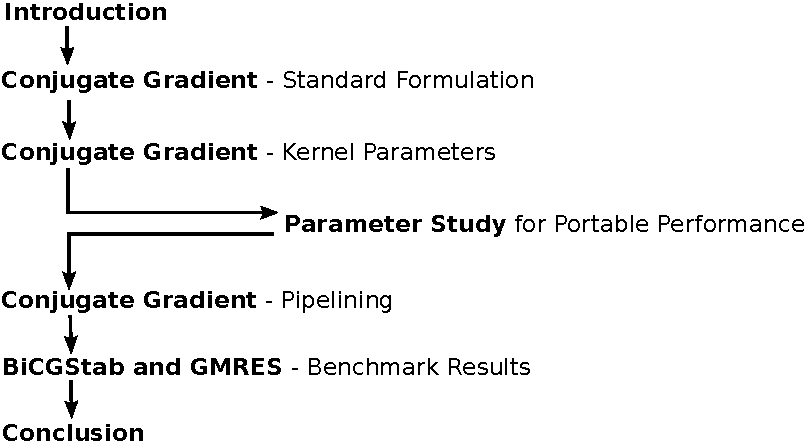
\includegraphics[width=0.9\textwidth]{figures/outline-crop}
 \end{center}
\end{frame}



\begin{frame}{Introduction}
  \begin{block}{Recent Many-Core Architectures}
    \begin{itemize}
     \item High FLOP/Watt ratio
     \item High memory bandwidth
     \item Attached via PCI-Express
    \end{itemize}
\vspace*{1cm}
  \end{block}

   \begin{minipage}{0.3\textwidth}
    \begin{center}
     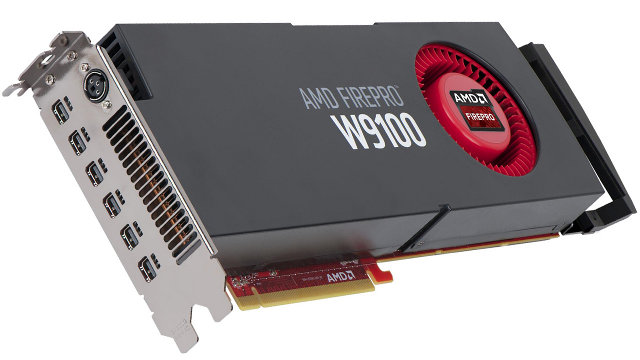
\includegraphics[width=0.99\textwidth]{figures/w9100.jpg} \\ AMD FirePro W9100 \\ 320 GB/sec
    \end{center}
   \end{minipage}
   \hspace{0.2cm}
%
   \begin{minipage}{0.3\textwidth}
    \begin{center}
     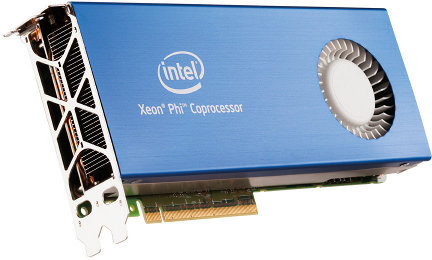
\includegraphics[width=0.92\textwidth]{figures/xeon-phi.jpg} \\ INTEL Xeon Phi \\ 320 (220?) GB/sec
    \end{center}
   \end{minipage}
   \hspace{0.2cm}
%
   \begin{minipage}{0.3\textwidth}
    \begin{center}
     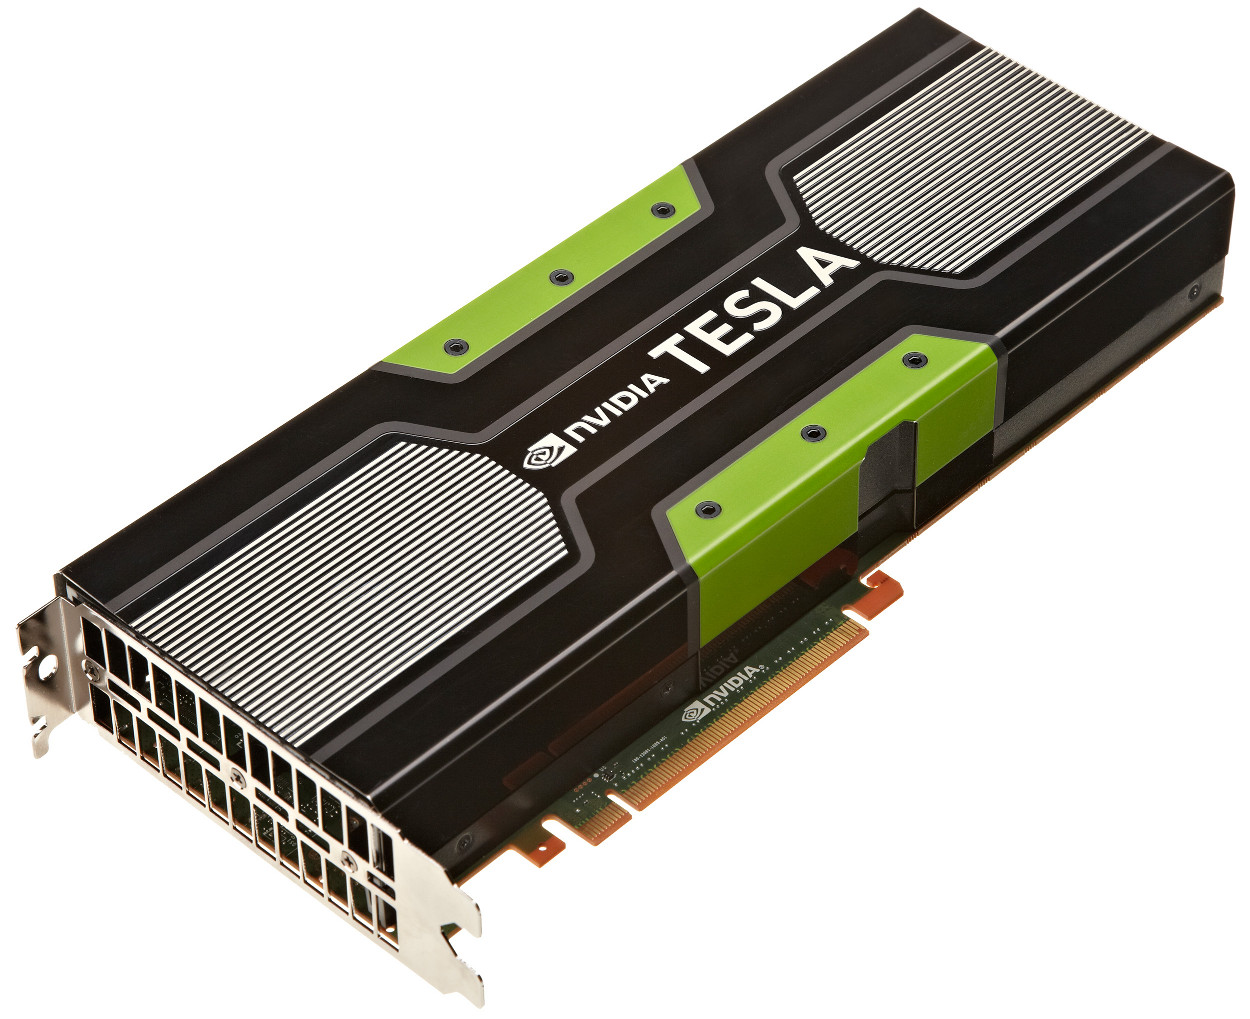
\includegraphics[width=0.7\textwidth]{figures/TeslaK20.jpg} \\ NVIDIA Tesla K20 \\ 250 (208) GB/sec
    \end{center}
   \end{minipage}


\end{frame}


\begin{frame}{Introduction}
 \vspace*{-0.5cm}
 \begin{center}
  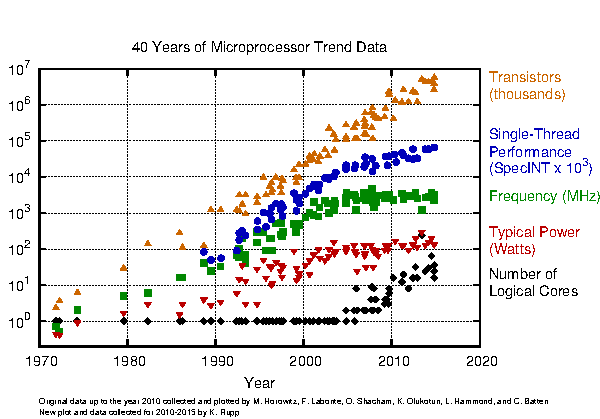
\includegraphics[width=0.95\textwidth]{figures/40-years-processor-trend}
 \end{center}
 {\tiny https://www.karlrupp.net/2015/06/40-years-of-microprocessor-trend-data/ }
\end{frame}

\begin{frame}{Introduction}
 \vspace*{-0.5cm}
 \begin{center}
  Theoretical Peak Performance \\
  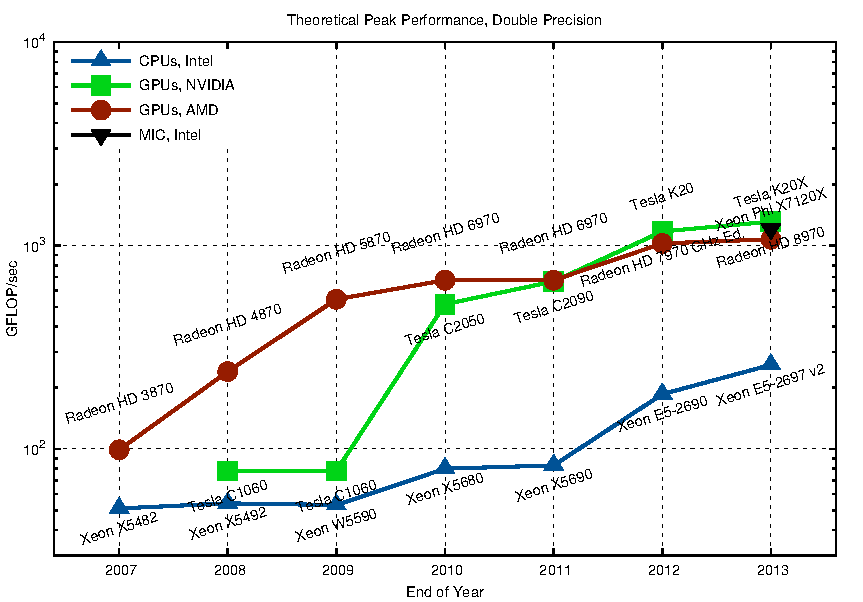
\includegraphics[width=0.95\textwidth]{figures/gflops-dp}
 \end{center}
 \vspace*{-0.5cm}
 {\tiny https://www.karlrupp.net/2013/06/cpu-gpu-and-mic-hardware-characteristics-over-time/ }
\end{frame}

\begin{frame}{Introduction}
 \vspace*{-0.5cm}
 \begin{center}
  Theoretical Peak Performance per Watt \\
  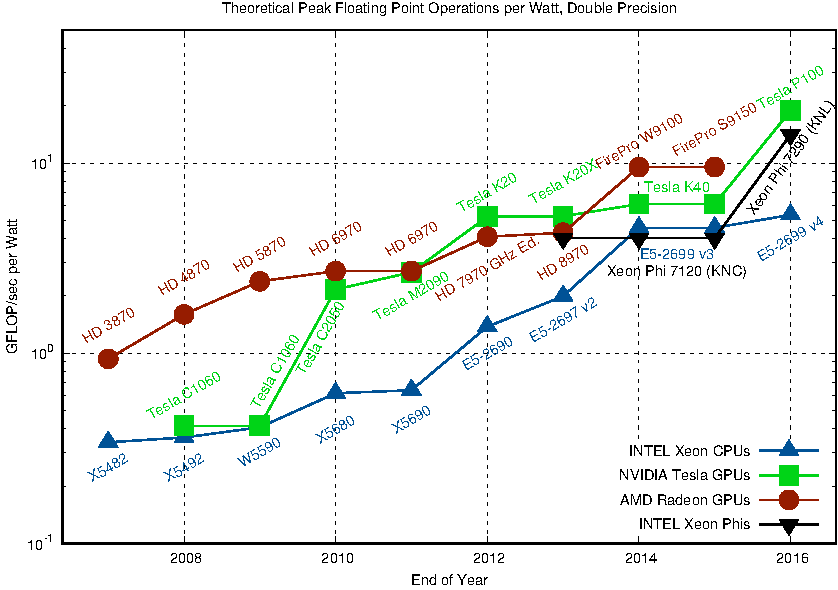
\includegraphics[width=0.95\textwidth]{figures/gflops-per-watt-dp}
 \end{center}
 \vspace*{-0.5cm}
 {\tiny https://www.karlrupp.net/2013/06/cpu-gpu-and-mic-hardware-characteristics-over-time/ }
\end{frame}

\begin{frame}{Introduction}
 \vspace*{-0.5cm}
 \begin{center}
  Theoretical Peak Performance (FLOPs) per Byte of Memory Bandwidth \\
  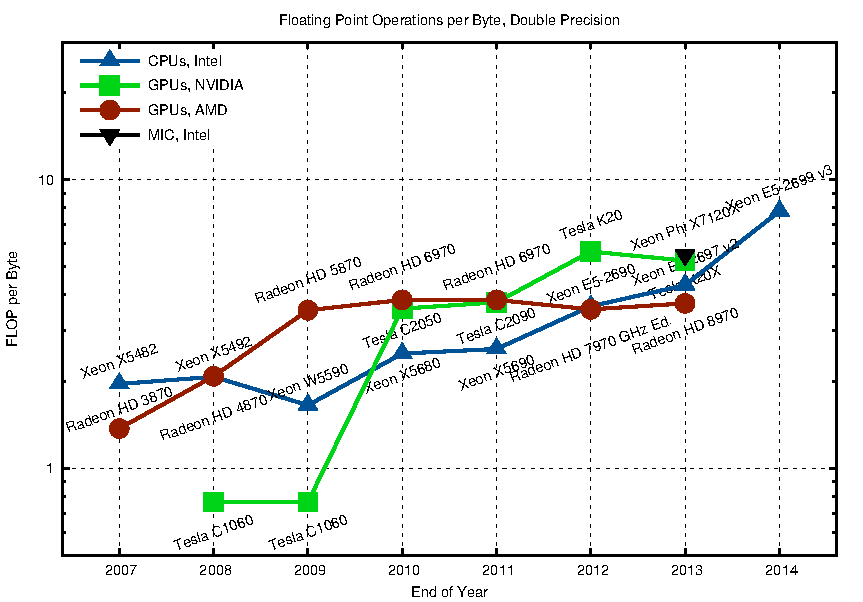
\includegraphics[width=0.95\textwidth]{figures/flop-per-byte-dp}
 \end{center}
 \vspace*{-0.5cm}
 {\tiny https://www.karlrupp.net/2013/06/cpu-gpu-and-mic-hardware-characteristics-over-time/ }
\end{frame}



%
% Introduce CG and perform first optimizations
%


%%
%% Conjugate Gradients: Pipelining
%%

% Show CG algorithm <-> BLAS


\begin{frame}[fragile]{Performance Modeling: Conjugate Gradients}

 \begin{block}{}
  
   \begin{minipage}{0.45\textwidth}
      {\large \textbf{Pseudocode}} \\
      
      Choose $x_0$ \\
      $p_0 = r_0 = b - Ax_0$ \\
      For $i=0$ until convergence
     \begin{enumerate}
      \item Compute and store $Ap_i$
      \item Compute $\langle p_i, Ap_i \rangle$
      \item $\alpha_i = \langle r_i, r_i \rangle / \langle p_i, Ap_i \rangle$
      \item $x_{i+1} = x_{i} + \alpha_i p_i$          
      \item $r_{i+1} = r_i - \alpha_i Ap_i$       
      \item Compute $\langle r_{i+1}, r_{i+1} \rangle$
      \item $\beta_i = \langle r_{i+1}, r_{i+1} \rangle / \langle r_i, r_i \rangle$
      \item $p_{i+1} = r_{i+1} + \beta_i p_i$
     \end{enumerate}
     EndFor
   \end{minipage}
   \begin{minipage}{0.48\textwidth}
      {\large \textbf{BLAS-based Implementation}} \\
      
            - \\
      SpMV, AXPY \\
      For $i=0$ until convergence
     \begin{enumerate}
      \item SpMV {\color{blue} $\leftarrow$ No caching of $Ap_i$}
      \item DOT {\color{red} $\leftarrow$ Global sync!}
      \item -
      \item AXPY         
      \item AXPY  {\color{blue} $\leftarrow$ No caching of $r_{i+1}$}
      \item DOT {\color{red} $\leftarrow$ Global sync!}
      \item -
      \item AXPY
     \end{enumerate}
     EndFor
   \end{minipage}
   
   \end{block}
   
\end{frame}

\begin{frame}[fragile]{Performance Modeling: Conjugate Gradients}

 \begin{block}{}
 
 \begin{center}
  \vspace*{-0.5cm}
  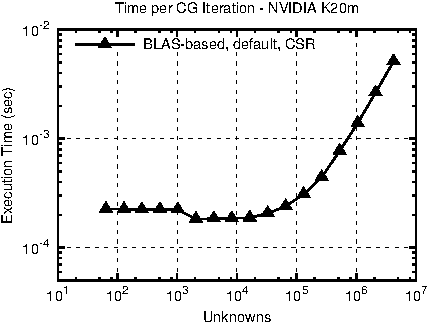
\includegraphics[width=0.85\textwidth]{figures/cg-k20m-0}
 \end{center}

 \begin{itemize}
  \item   \vspace*{-0.3cm} {\small (Poisson, 2D, Finite Differences)}
 \end{itemize}

 \end{block}
   
\end{frame}


\begin{frame}[fragile]{Performance Modeling: Conjugate Gradients}

 \begin{block}{Performance Modelling}
   \begin{itemize}
    \item 6 Kernel Launches (plus two for reductions)
    \item Two device to host data reads from dot products
    \item Model SpMV as seven vector accesses (5-point stencil)
    \item $T(N) = 8 \times 10^{-6} + 2 \times 2 \times 10^{-6} + (7+2+3+3+2+3) \times 8 \times N / \mathrm{Bandwidth}$
   \end{itemize}

 %\pause
 \begin{center}
  \vspace*{-0.2cm}
  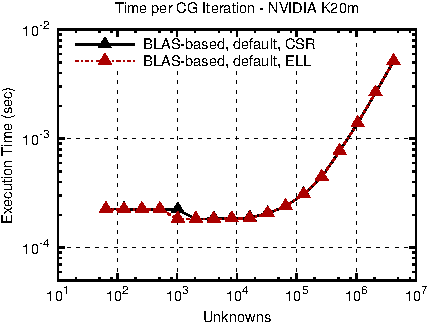
\includegraphics[width=0.65\textwidth]{figures/cg-k20m-1}
 \end{center}

%  \begin{itemize}
%   \item   \vspace*{-0.5cm} {\small (Poisson, 2D, Finite Differences)}
%  \end{itemize}

 \end{block}
   
\end{frame}


%%%%%%%%

% Step 3: Show and discuss pipelined/improved version

\begin{frame}[fragile]{Performance Modeling: Conjugate Gradient Optimizations}

 \begin{block}{Optimization: Rearrange the algorithm}
   \begin{itemize}
   \item  Remove unnecessary reads 
   \item  Remove unnecessary synchronizations
   \item Use custom kernels instead of standard BLAS
  \end{itemize}
 \end{block}
   
\end{frame}



\begin{frame}[fragile]{Performance Modeling: Conjugate Gradients}

 \begin{block}{}
  
   \begin{minipage}{0.45\textwidth}
      {\large \textbf{Standard CG}} \\
      
      Choose $x_0$ \\
      $p_0 = r_0 = b - Ax_0$ \\
      For $i=0$ until convergence
     \begin{enumerate}
      \item Compute and store $Ap_i$
      \item Compute $\langle p_i, Ap_i \rangle$
      \item $\alpha_i = \langle r_i, r_i \rangle / \langle p_i, Ap_i \rangle$
      \item $x_{i+1} = x_{i} + \alpha_i p_i$          
      \item $r_{i+1} = r_i - \alpha_i Ap_i$       
      \item Compute $\langle r_{i+1}, r_{i+1} \rangle$
      \item $\beta_i = \langle r_{i+1}, r_{i+1} \rangle / \langle r_i, r_i \rangle$
      \item $p_{i+1} = r_{i+1} + \beta_i p_i$
     \end{enumerate}
     EndFor
   \end{minipage}
   \begin{minipage}{0.53\textwidth}
      {\large \textbf{Pipelined CG}} \\
      
      Choose $x_0$ \\
      $p_0 = r_0 = b - Ax_0$ \\
      For $i=1$ until convergence
     \begin{enumerate}
      \item $i=1$: Compute $\alpha_0$, $\beta_0$, $Ap_0$
      \item {\color{blue}$x_i = x_{i-1} + \alpha_{i-1} p_{i-1}$}
      \item {\color{blue}$r_i = r_{i-1} - \alpha_{i-1} Ap_i$}
      \item {\color{blue}$p_i = r_i + \beta_{i-1} p_{i-1}$}       
      \item {\color{red} Compute and store $Ap_i$}
      \item  {\color{red} Compute $\langle Ap_i, Ap_i \rangle$, $\langle p_i, Ap_i \rangle$}, {\color{blue}$\langle r_i, r_i \rangle$}
      \item $\alpha_i = \langle r_i, r_i \rangle / \langle p_i, Ap_i \rangle$
      \item $\beta_i = ( \alpha_i^2 \langle Ap_i, Ap_i \rangle - \langle r_i, r_i \rangle) / \langle r_i, r_i \rangle$
     \end{enumerate}
     EndFor
   \end{minipage}
   
   \end{block}
   
\end{frame}


\begin{frame}[fragile]{Performance Modeling: Conjugate Gradients}
 \begin{block}{}
 \begin{center}
  \vspace*{-0.5cm}
  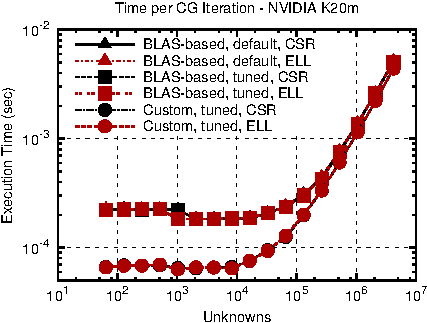
\includegraphics[width=0.85\textwidth]{figures/cg-k20m-3}
 \end{center}

 \begin{itemize}
  \item   \vspace*{-0.3cm} {\small (Poisson, 2D, Finite Differences)}
 \end{itemize}
 \end{block}   
\end{frame}



\begin{frame}[fragile]{Performance Modeling: Conjugate Gradients}
 \begin{block}{Benefits of Pipelining also for Large Matrices}
 \begin{center}
  \vspace*{-0.2cm}
  \hspace*{-1.5cm}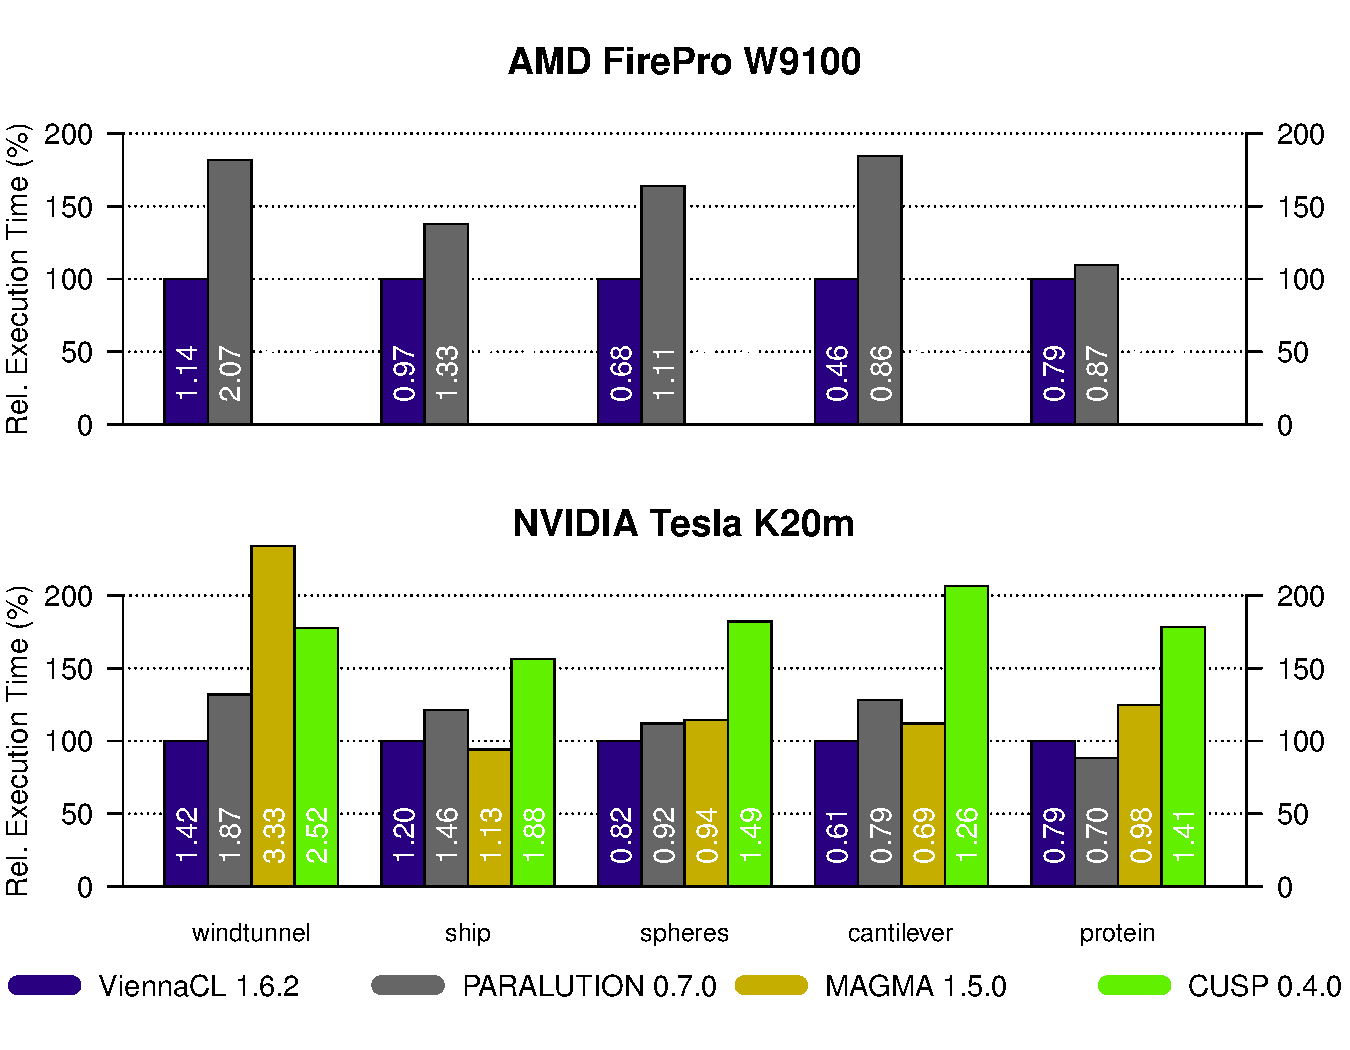
\includegraphics[width=1.05\textwidth]{figures/cg}
 \end{center}
  \vspace*{0.2cm}

 \end{block}   
\end{frame}




%
% Parameter Tuning: Explain benchmark setting, then present results
%


\begin{frame}{Benchmark Setting}

  \begin{block}{Scope for OpenCL-based Portability Study}
    \begin{itemize}
     \item Vector and matrix-vector operations (BLAS levels 1 and 2)
     \item Limited by memory bandwidth
     %\item Matrix-matrix-multiplication (only briefly today)
    \end{itemize}
  \end{block}

  \pause
  \begin{block}{Key Question (Memory-Bandwidth-Limited Kernels)}
    \begin{center} \color{red} \LARGE
     Good performance of complicated kernels \\
     by optimizing the simplest kernel?
    \end{center}
  \end{block}

\end{frame}


%% Copy kernel:
\begin{frame}[fragile]{Benchmark Setting}
  \begin{block}{Vector Assignment (Copy) Kernel}
    \begin{itemize}
     \item $x \Leftarrow y$ for (large) vectors $x$, $y$
    \end{itemize}
  \end{block}

  \only<1>{\begin{center} \vspace*{0.85cm} 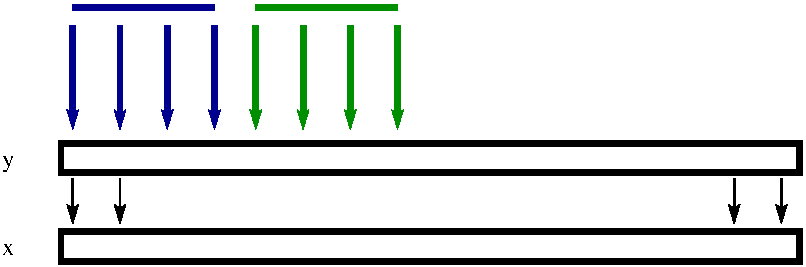
\includegraphics[width=0.8\textwidth]{figures/copy-kernel-gpu-1} \end{center}}
  \only<2>{\begin{center}                  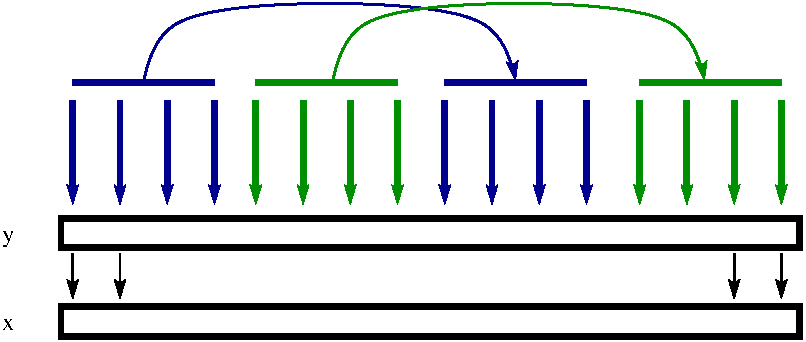
\includegraphics[width=0.8\textwidth]{figures/copy-kernel-gpu-full} \end{center}}
  \only<3>{\begin{center} \vspace*{0.84cm} 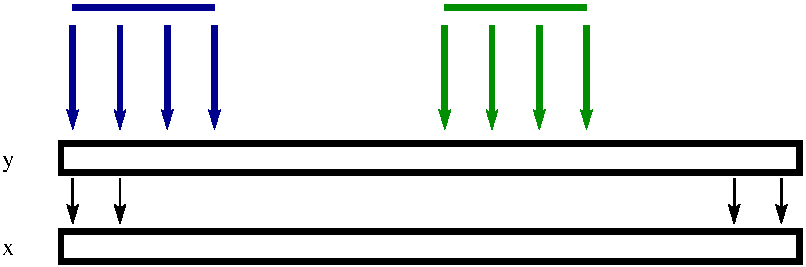
\includegraphics[width=0.8\textwidth]{figures/copy-kernel-cpu-1} \end{center}}
  \only<4>{\begin{center} \vspace*{0.30cm} 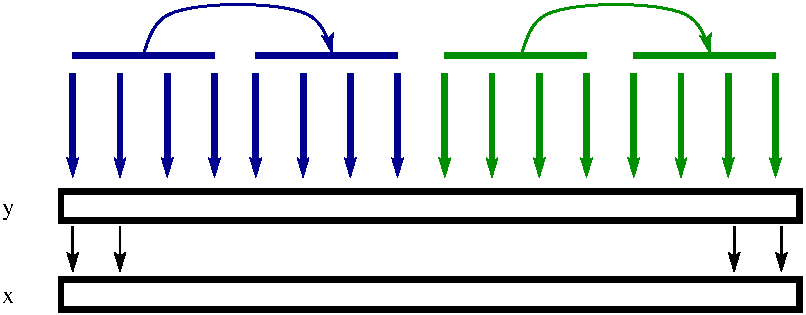
\includegraphics[width=0.8\textwidth]{figures/copy-kernel-cpu-full} \end{center}}
  
  \only<1>{
  \begin{block}{Parameters (1900 variations) }
   \begin{itemize}
    \item Local work size, global work size
    \item Vector types (float1, float2, ... , float16)
    \item Thread increment type
   \end{itemize}
  \end{block}}
  
  \only<2>{
  \begin{block}{Parameters (1900 variations) }
   \begin{itemize}
     \item \texttt{for (size\_t i = get\_global\_id(0); i < N;}
     \item \texttt{\ \ \ \ \ \ \ \ \ \ \ \ i+= get\_global\_size(0))}
     \item \texttt{\ \ x[i] = y[i];}
   \end{itemize}
  \end{block}
  }

  \only<3>{
  \begin{block}{Parameters (1900 variations) }
   \begin{itemize}
     \item \texttt{for (size\_t i = group\_start + get\_local\_id(0);}
     \item \texttt{\ \ \ \ \ i < group\_end; i+= get\_local\_size(0)) }
     \item \texttt{\ \  x[i] = y[i];}
   \end{itemize}
  \end{block}
  }

  \only<4>{
  \begin{block}{Parameters (1900 variations) }
   \begin{itemize}
     \item \texttt{for (size\_t i = group\_start + get\_local\_id(0);}
     \item \texttt{\ \ \ \ \ i < group\_end; i+= get\_local\_size(0)) }
     \item \texttt{\ \  x[i] = y[i];}
   \end{itemize}
  \end{block}
  }
\end{frame}


%% 
\begin{frame}{Benchmark Setting}

  \begin{block}{Operations}
   \begin{itemize}
    \item Vector copy, vector addition, inner product
    \item Matrix-vector product
   \end{itemize}
  \end{block}

  %\only<1>{\begin{center} 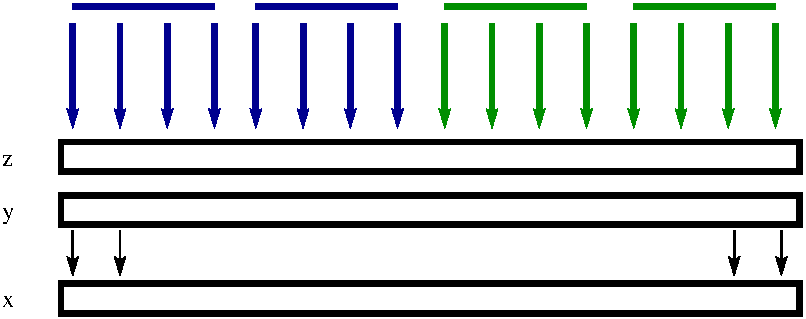
\includegraphics[width=0.8\textwidth]{figures/addition-kernel} \end{center}}
  %\only<2>{\begin{center} 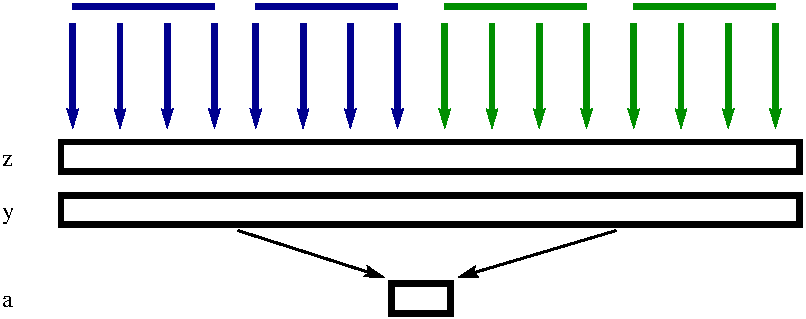
\includegraphics[width=0.8\textwidth]{figures/inner-product-kernel} \end{center}}

  %\visible<3->{
  \begin{center} 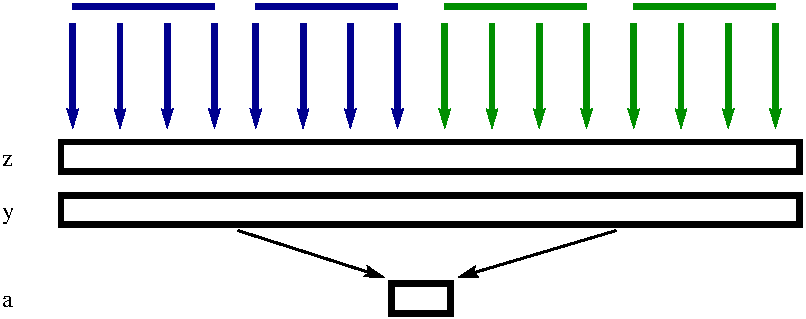
\includegraphics[width=0.8\textwidth]{figures/inner-product-kernel} \end{center}

  \begin{block}{Devices}
   \begin{itemize}
    \item AMD: A10-5800 APU, HD 5850 GPU
    \item INTEL: Dual Socket Xeon E5-2670, Xeon Phi
    \item NVIDIA: GTX 285, Tesla K20m
   \end{itemize}
  \end{block}
  %}
  
\end{frame}



\begin{frame}{Portable Performance}
  \begin{center} \Large \textbf{Histograms} \end{center}
\end{frame}

\begin{frame}{Portable Performance}
  \begin{center} 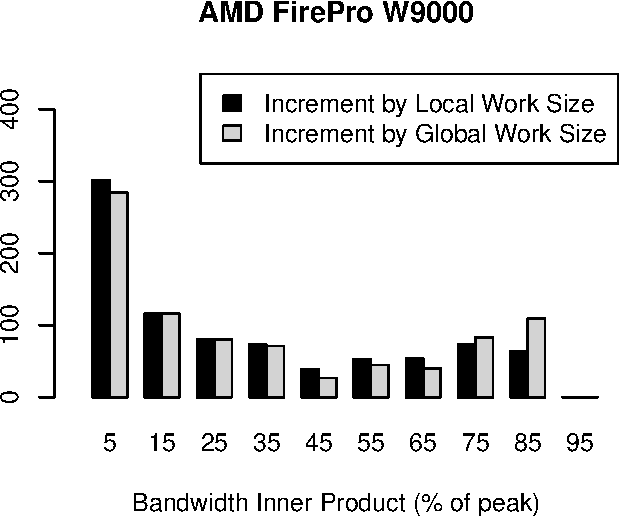
\includegraphics[width=0.75\textwidth]{figures/firepro_w9000_double_hist_itertype_dot} \end{center}
\end{frame}

\begin{frame}{Portable Performance}
  \begin{center} 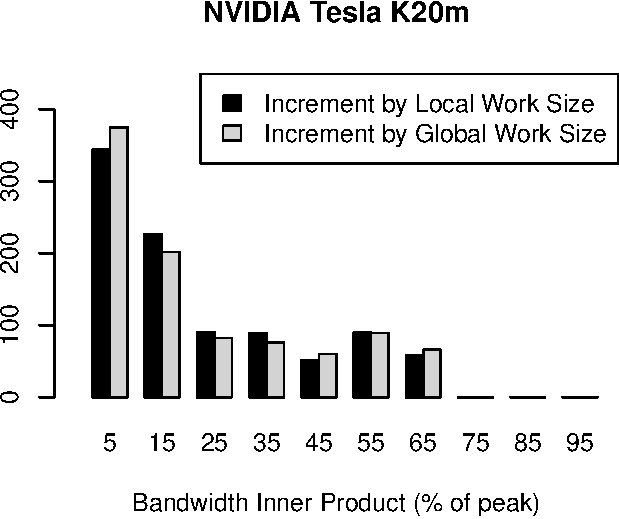
\includegraphics[width=0.75\textwidth]{figures/k20m_double_hist_itertype_dot} \end{center}
\end{frame}

\begin{frame}{Portable Performance}
  \begin{center} 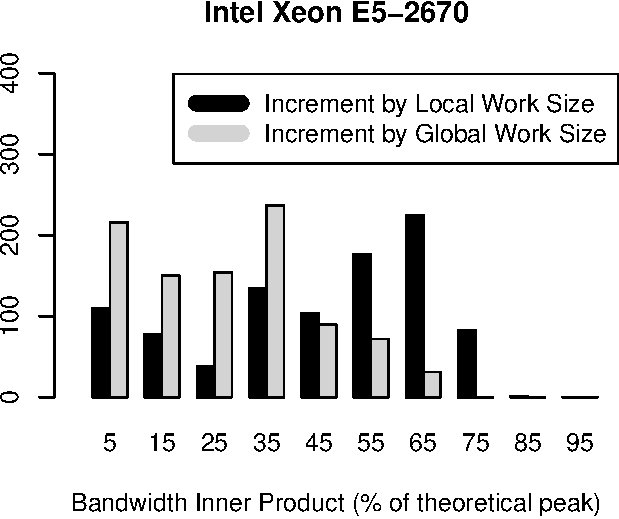
\includegraphics[width=0.75\textwidth]{figures/xeon_cpu_double_hist_itertype_dot} \end{center}
\end{frame}

\begin{frame}{Portable Performance}
  \begin{center} 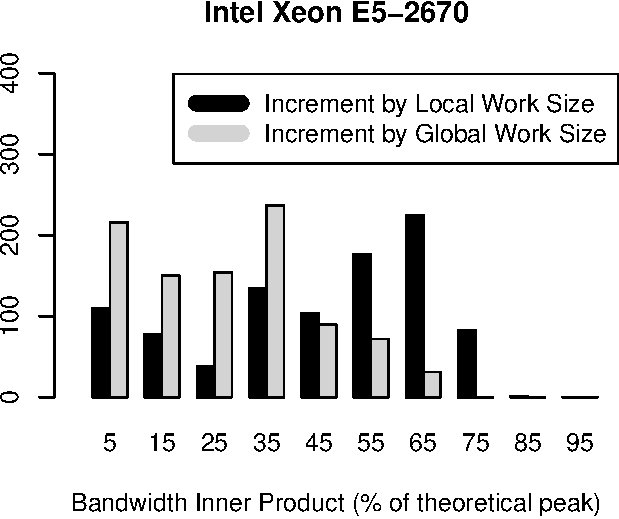
\includegraphics[width=0.55\textwidth]{figures/xeon_cpu_double_hist_itertype_dot} \\[1em]
                 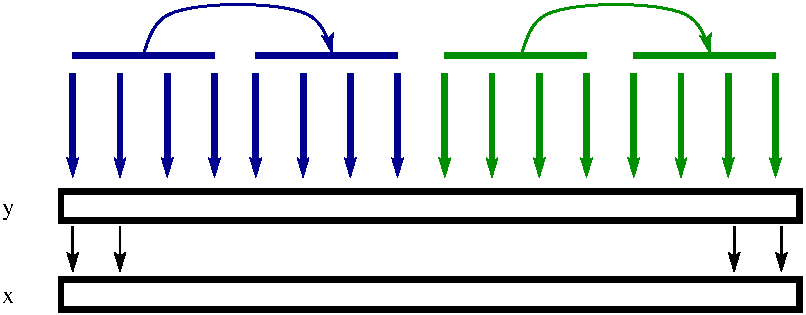
\includegraphics[width=0.45\textwidth]{figures/copy-kernel-cpu-full} 
  \end{center}
\end{frame}


%%%%%%%%%%%%%%%%%%%%%%%%%%%%%%%%%%%%%%%%%%%%%%%%%%%%%%%%%%%%%%%


\begin{frame}{Portable Performance}
  \begin{center} \textbf{ [Addition$|$Inner Product$|$Matrix-Vector] vs. Copy Kernel }\\[1em] Same Device \end{center}
\end{frame}

\begin{frame}{Portable Performance}
  \only<1>{\begin{center} 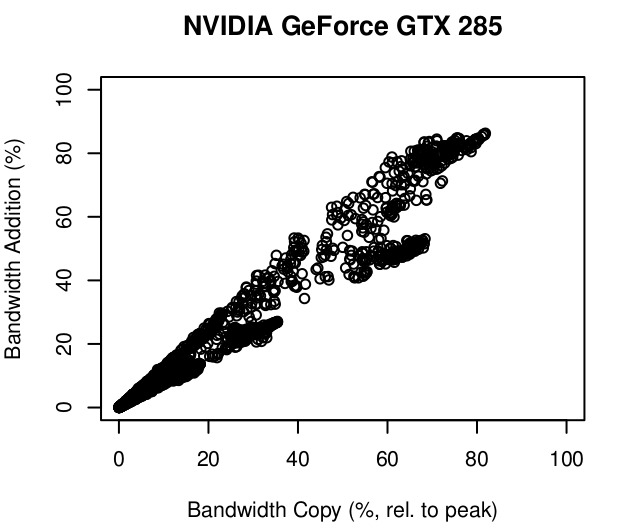
\includegraphics[width=0.8\textwidth]{figures/gtx285-addition-copy-1} \end{center}}
  \only<2>{\begin{center} 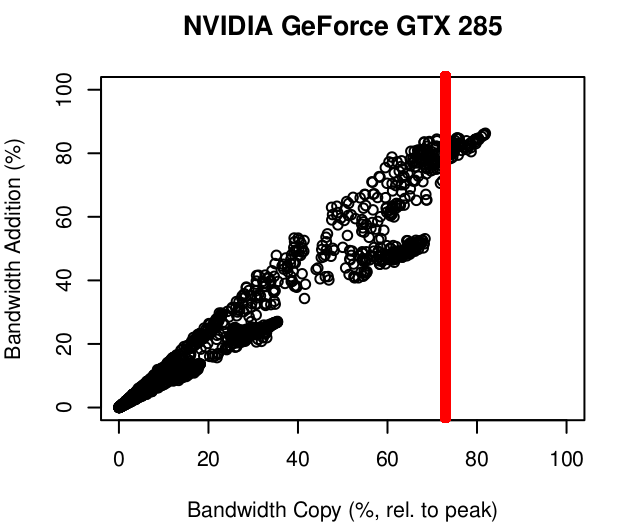
\includegraphics[width=0.8\textwidth]{figures/gtx285-addition-copy-2} \end{center}}
  \only<3>{\begin{center} 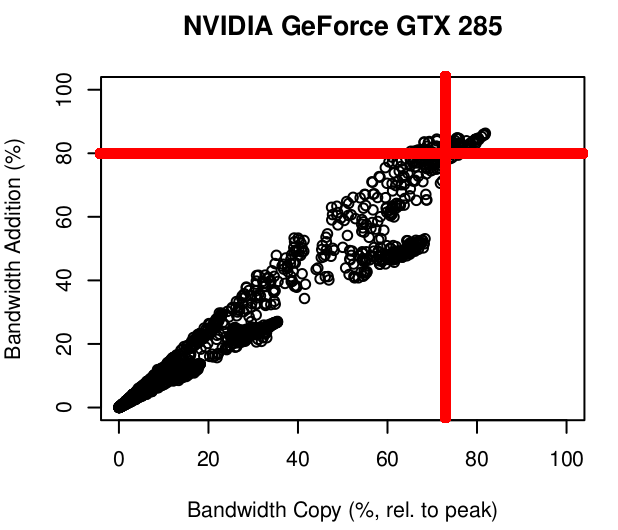
\includegraphics[width=0.8\textwidth]{figures/gtx285-addition-copy-3} \end{center}}
\end{frame}


\begin{frame}{Portable Performance}
  \only<1>{\begin{center} {\LARGE NVIDIA Tesla K20m} \\[2em]       \hspace*{1.cm} Addition \hspace*{2.1cm} Inner Product \hspace*{1.4cm} Mat-Vec Product \\[1em] 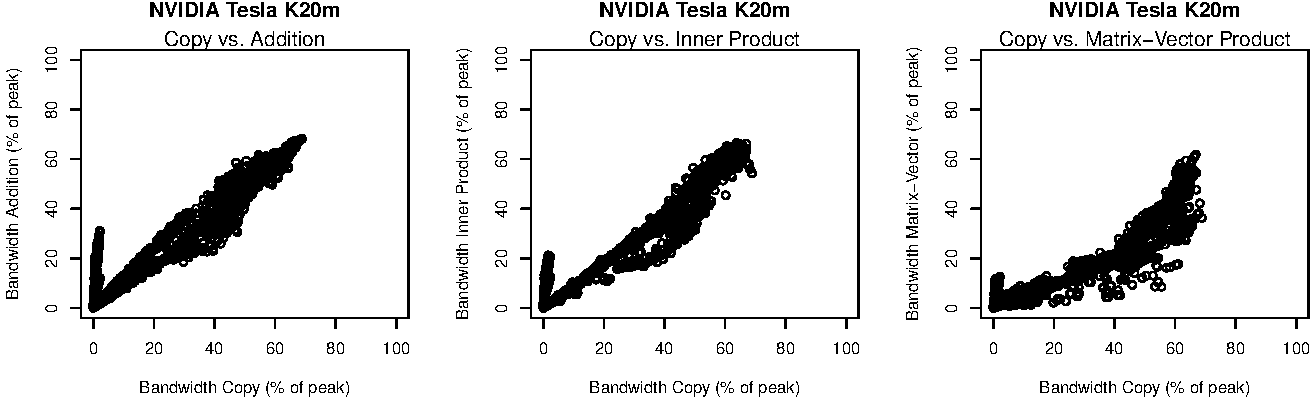
\includegraphics[width=0.99\textwidth]{figures/k20m_double_xy_copy-crop} \end{center}}
  \only<2>{\begin{center} {\LARGE AMD Radeon HD 5850} \\[2em]      \hspace*{1.cm} Addition \hspace*{2.1cm} Inner Product \hspace*{1.4cm} Mat-Vec Product \\[1em] 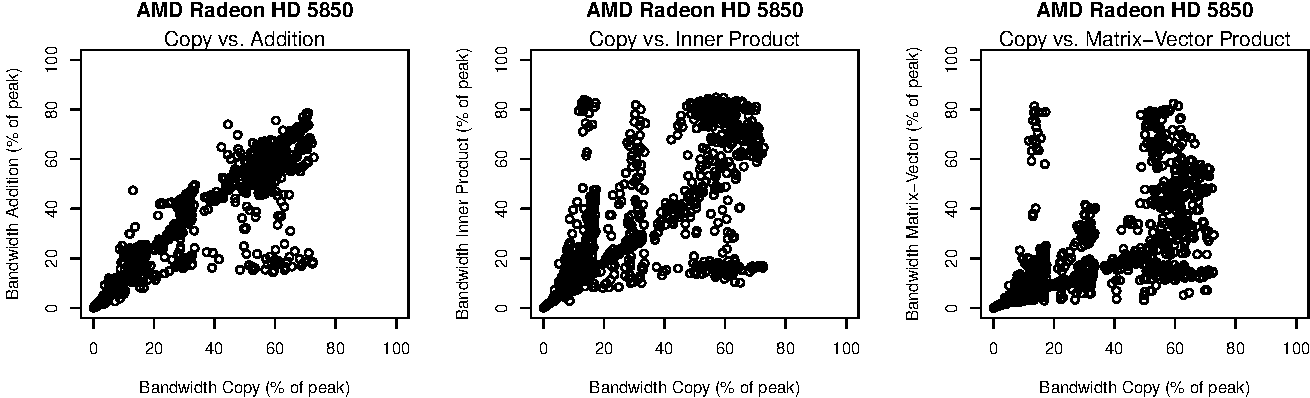
\includegraphics[width=0.99\textwidth]{figures/hd5850_double_xy_copy-crop} \end{center}}
  \only<3>{\begin{center} {\LARGE AMD FirePro W9000} \\[2em]       \hspace*{1.cm} Addition \hspace*{2.1cm} Inner Product \hspace*{1.4cm} Mat-Vec Product \\[1em] 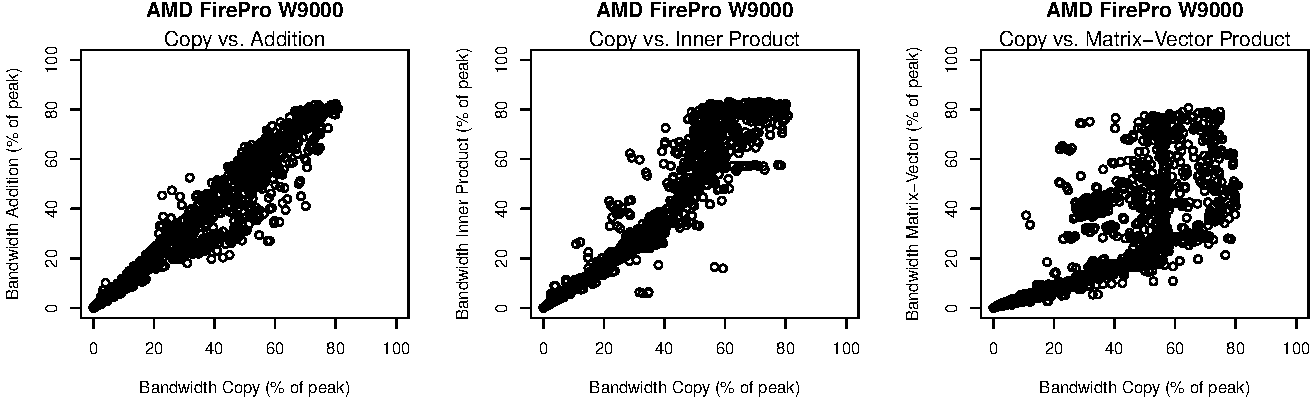
\includegraphics[width=0.99\textwidth]{figures/firepro_w9000_double_xy_copy} \end{center}}
  \only<4>{\begin{center} {\LARGE INTEL Dual Xeon E5-2670} \\[2em] \hspace*{1.cm} Addition \hspace*{2.1cm} Inner Product \hspace*{1.4cm} Mat-Vec Product \\[1em] 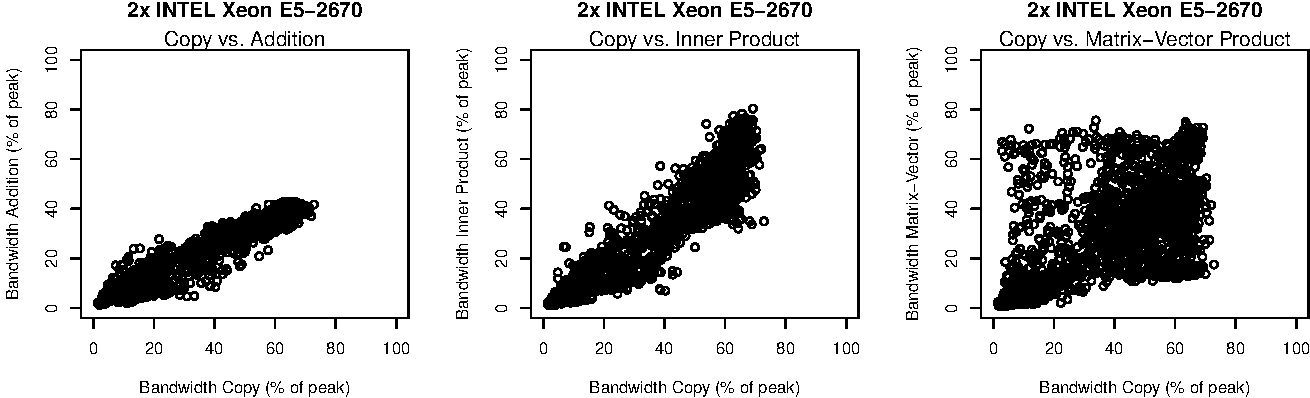
\includegraphics[width=0.99\textwidth]{figures/xeon_cpu_double_xy_copy-crop} \end{center}}
  \only<5>{\begin{center} {\LARGE INTEL Xeon Phi} \\[2em]          \hspace*{1.cm} Addition \hspace*{2.1cm} Inner Product \hspace*{1.4cm} Mat-Vec Product \\[1em] 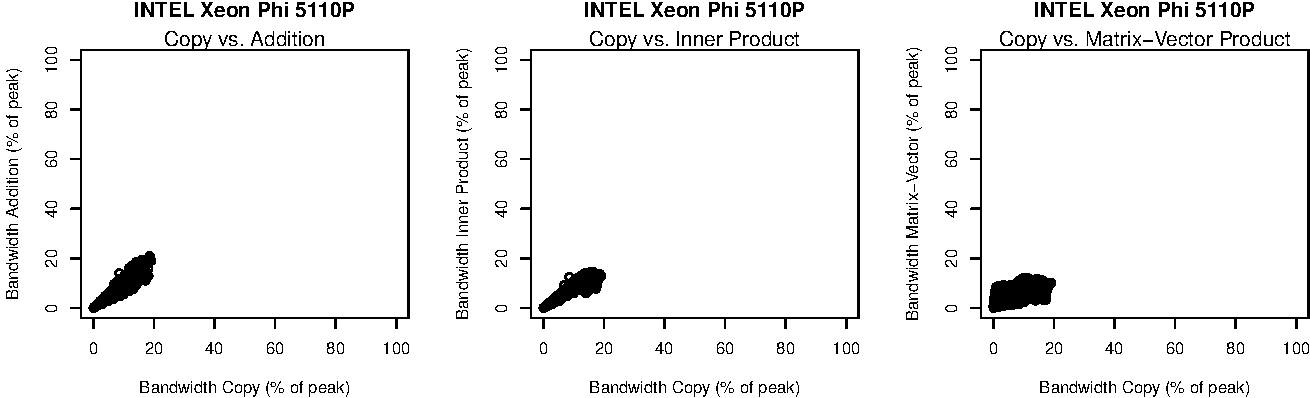
\includegraphics[width=0.99\textwidth]{figures/xeon_phi_float_xy_copy-crop} \end{center}}
\end{frame}

\begin{frame}{Portable Performance}
  \begin{center} Conclusio: \\[1em]
    {\Large Focus on fastest configurations for copy-kernel sufficient} \\[5em]
    
    Good choice: \\[1em]
    {\Large Local workgroup size of 128 with 128 workgroups}
  \end{center}
\end{frame}



%%%%%%%%%%%%%%%%%%%%%%%%%%%%%%%%%%%%%%%%%%%%%%%%%%%%%%%%%%%%%%%



\begin{frame}{Portable Performance}
  \begin{block}{Matrix-Matrix Multiplication}
    \begin{itemize}
     \item Compute-bound
     \item Block-decomposition to maximize cache utilization
    \end{itemize}
  \end{block}
  
  \begin{center}
   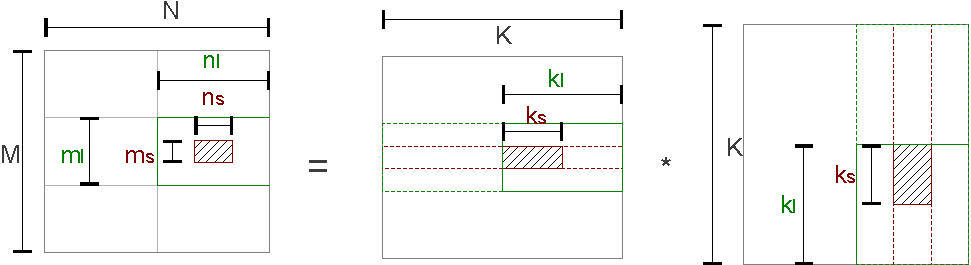
\includegraphics[width=0.99\textwidth]{figures/MatrixMatrixProduct}
  \end{center}


\end{frame}


\begin{frame}{Portable Performance}
  \begin{center}
  Matrix-Matrix Multiplication (Single Precision) \\
  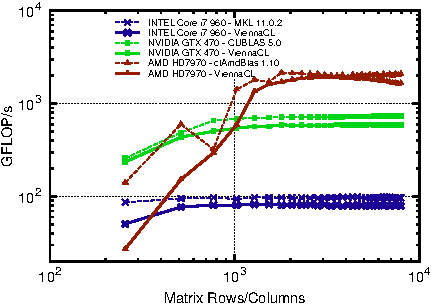
\includegraphics[width=0.8\textwidth]{figures/sgemm}
  \end{center} 
  
  {\small Ph.~Tillet \textit{et al.}: HotPar'13}
\end{frame}



%
% Continue with CG-method, show results for pipelined variant
%


\begin{frame}{Outline}
 \begin{center}
  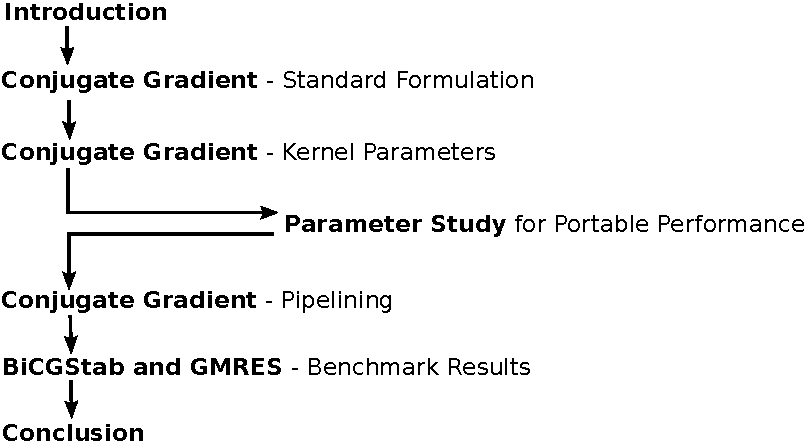
\includegraphics[width=0.9\textwidth]{figures/outline-crop}
 \end{center}
\end{frame}

\begin{frame}[fragile]{Conjugate Gradients}
 \begin{block}{}
 \begin{center}
  \vspace*{-0.5cm}
  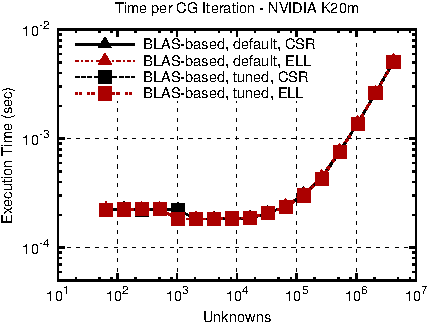
\includegraphics[width=0.85\textwidth]{figures/cg-k20m-2}
 \end{center}

 \begin{itemize}
  \item   \vspace*{-0.3cm} {\small (2D Finite Difference Discretization)}
 \end{itemize}
 \end{block}   
\end{frame}

\begin{frame}[fragile]{Conjugate Gradients}
 \begin{block}{}
 \begin{center}
  \vspace*{-0.5cm}
  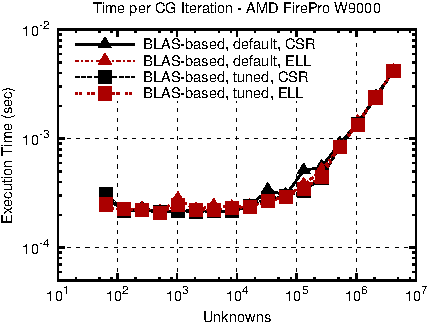
\includegraphics[width=0.85\textwidth]{figures/cg-firepro-w9000-2}
 \end{center}

 \begin{itemize}
  \item   \vspace*{-0.3cm} {\small (2D Finite Difference Discretization)}
 \end{itemize}
 \end{block}   
\end{frame}


% Step 3: Show and discuss pipelined/improved version

\begin{frame}[fragile]{Conjugate Gradient Optimizations}

 \begin{block}{Optimization 3: Rearrange the algorithm}
   \begin{itemize}
   \item  Remove unnecessary reads 
   \item  Remove unnecessary synchronizations
   \item Use custom kernels instead of standard BLAS
  \end{itemize}
 \end{block}
   
\end{frame}


\begin{frame}[fragile]{Conjugate Gradients}

 \begin{block}{}
  
   \begin{minipage}{0.45\textwidth}
      {\large \textbf{Standard CG}} \\
      
      Choose $x_0$ \\
      $p_0 = r_0 = b - Ax_0$ \\
      For $i=0$ until convergence
     \begin{enumerate}
      \item Compute and store $Ap_i$
      \item Compute $\langle p_i, Ap_i \rangle$
      \item $\alpha_i = \langle r_i, r_i \rangle / \langle p_i, Ap_i \rangle$
      \item $x_{i+1} = x_{i} + \alpha_i p_i$          
      \item $r_{i+1} = r_i - \alpha_i Ap_i$       
      \item Compute $\langle r_{i+1}, r_{i+1} \rangle$
      \item $\beta_i = \langle r_{i+1}, r_{i+1} \rangle / \langle r_i, r_i \rangle$
      \item $p_{i+1} = r_{i+1} + \beta_i p_i$
     \end{enumerate}
     EndFor
   \end{minipage}
   \begin{minipage}{0.53\textwidth}
   \end{minipage}
   
   \end{block}
   
\end{frame}


\begin{frame}[fragile]{Conjugate Gradients}

 \begin{block}{}
  
   \begin{minipage}{0.45\textwidth}
      {\large \textbf{Standard CG}} \\
      
      Choose $x_0$ \\
      $p_0 = r_0 = b - Ax_0$ \\
      For $i=0$ until convergence
     \begin{enumerate}
      \item Compute and store $Ap_i$
      \item Compute $\langle p_i, Ap_i \rangle$
      \item $\alpha_i = \langle r_i, r_i \rangle / \langle p_i, Ap_i \rangle$
      \item $x_{i+1} = x_{i} + \alpha_i p_i$          
      \item $r_{i+1} = r_i - \alpha_i Ap_i$       
      \item Compute $\langle r_{i+1}, r_{i+1} \rangle$
      \item $\beta_i = \langle r_{i+1}, r_{i+1} \rangle / \langle r_i, r_i \rangle$
      \item $p_{i+1} = r_{i+1} + \beta_i p_i$
     \end{enumerate}
     EndFor
   \end{minipage}
   \begin{minipage}{0.53\textwidth}
      {\large \textbf{Pipelined CG}} \\
      
      Choose $x_0$ \\
      $p_0 = r_0 = b - Ax_0$ \\
      For $i=1$ until convergence
     \begin{enumerate}
      \item $i=1$: Compute $\alpha_0$, $\beta_0$, $Ap_0$
      \item $x_i = x_{i-1} + \alpha_{i-1} p_{i-1}$          
      \item $r_i = r_{i-1} - \alpha_{i-1} Ap_i$       
      \item $p_i = r_i + \beta_{i-1} p_{i-1}$       
      \item Compute and store $Ap_i$
      \item Compute $\langle Ap_i, Ap_i \rangle$, $\langle p_i, Ap_i \rangle$, $\langle r_i, r_i \rangle$
      \item $\alpha_i = \langle r_i, r_i \rangle / \langle p_i, Ap_i \rangle$
      \item $\beta_i = ( \alpha_i^2 \langle Ap_i, Ap_i \rangle - \langle r_i, r_i \rangle) / \langle r_i, r_i \rangle$
     \end{enumerate}
     EndFor
   \end{minipage}
   
   \end{block}
   
\end{frame}

\begin{frame}[fragile]{Conjugate Gradients}

 \begin{block}{}
  
   \begin{minipage}{0.45\textwidth}
      {\large \textbf{Standard CG}} \\
      
      Choose $x_0$ \\
      $p_0 = r_0 = b - Ax_0$ \\
      For $i=0$ until convergence
     \begin{enumerate}
      \item Compute and store $Ap_i$
      \item Compute $\langle p_i, Ap_i \rangle$
      \item $\alpha_i = \langle r_i, r_i \rangle / \langle p_i, Ap_i \rangle$
      \item $x_{i+1} = x_{i} + \alpha_i p_i$          
      \item $r_{i+1} = r_i - \alpha_i Ap_i$       
      \item Compute $\langle r_{i+1}, r_{i+1} \rangle$
      \item $\beta_i = \langle r_{i+1}, r_{i+1} \rangle / \langle r_i, r_i \rangle$
      \item $p_{i+1} = r_{i+1} + \beta_i p_i$
     \end{enumerate}
     EndFor
   \end{minipage}
   \begin{minipage}{0.53\textwidth}
      {\large \textbf{Pipelined CG}} \\
      
      Choose $x_0$ \\
      $p_0 = r_0 = b - Ax_0$ \\
      For $i=1$ until convergence
     \begin{enumerate}
      \item $i=1$: Compute $\alpha_0$, $\beta_0$, $Ap_0$
      \item {\color{blue}$x_i = x_{i-1} + \alpha_{i-1} p_{i-1}$}
      \item {\color{blue}$r_i = r_{i-1} - \alpha_{i-1} Ap_i$}
      \item {\color{blue}$p_i = r_i + \beta_{i-1} p_{i-1}$}       
      \item Compute and store $Ap_i$
      \item Compute $\langle Ap_i, Ap_i \rangle$, $\langle p_i, Ap_i \rangle$, {\color{blue}$\langle r_i, r_i \rangle$}
      \item $\alpha_i = \langle r_i, r_i \rangle / \langle p_i, Ap_i \rangle$
      \item $\beta_i = ( \alpha_i^2 \langle Ap_i, Ap_i \rangle - \langle r_i, r_i \rangle) / \langle r_i, r_i \rangle$
     \end{enumerate}
     EndFor
   \end{minipage}
   
   \end{block}
   
\end{frame}


\begin{frame}[fragile]{Conjugate Gradients}

 \begin{block}{}
  
   \begin{minipage}{0.45\textwidth}
      {\large \textbf{Standard CG}} \\
      
      Choose $x_0$ \\
      $p_0 = r_0 = b - Ax_0$ \\
      For $i=0$ until convergence
     \begin{enumerate}
      \item Compute and store $Ap_i$
      \item Compute $\langle p_i, Ap_i \rangle$
      \item $\alpha_i = \langle r_i, r_i \rangle / \langle p_i, Ap_i \rangle$
      \item $x_{i+1} = x_{i} + \alpha_i p_i$          
      \item $r_{i+1} = r_i - \alpha_i Ap_i$       
      \item Compute $\langle r_{i+1}, r_{i+1} \rangle$
      \item $\beta_i = \langle r_{i+1}, r_{i+1} \rangle / \langle r_i, r_i \rangle$
      \item $p_{i+1} = r_{i+1} + \beta_i p_i$
     \end{enumerate}
     EndFor
   \end{minipage}
   \begin{minipage}{0.53\textwidth}
      {\large \textbf{Pipelined CG}} \\
      
      Choose $x_0$ \\
      $p_0 = r_0 = b - Ax_0$ \\
      For $i=1$ until convergence
     \begin{enumerate}
      \item $i=1$: Compute $\alpha_0$, $\beta_0$, $Ap_0$
      \item {\color{blue}$x_i = x_{i-1} + \alpha_{i-1} p_{i-1}$}
      \item {\color{blue}$r_i = r_{i-1} - \alpha_{i-1} Ap_i$}
      \item {\color{blue}$p_i = r_i + \beta_{i-1} p_{i-1}$}       
      \item {\color{red} Compute and store $Ap_i$}
      \item  {\color{red} Compute $\langle Ap_i, Ap_i \rangle$, $\langle p_i, Ap_i \rangle$}, {\color{blue}$\langle r_i, r_i \rangle$}
      \item $\alpha_i = \langle r_i, r_i \rangle / \langle p_i, Ap_i \rangle$
      \item $\beta_i = ( \alpha_i^2 \langle Ap_i, Ap_i \rangle - \langle r_i, r_i \rangle) / \langle r_i, r_i \rangle$
     \end{enumerate}
     EndFor
   \end{minipage}
   
   \end{block}
   
\end{frame}


\begin{frame}[fragile]{Conjugate Gradients}
 \begin{block}{}
 \begin{center}
  \vspace*{-0.5cm}
  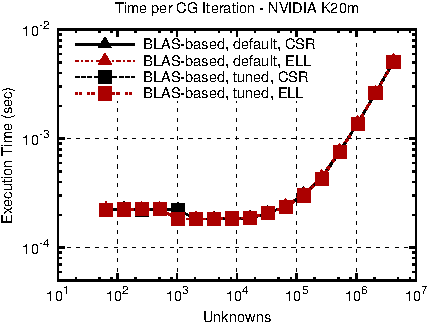
\includegraphics[width=0.85\textwidth]{figures/cg-k20m-2}
 \end{center}

 \begin{itemize}
  \item   \vspace*{-0.3cm} {\small (2D Finite Difference Discretization)}
 \end{itemize}
 \end{block}   
\end{frame}

\begin{frame}[fragile]{Conjugate Gradients}
 \begin{block}{}
 \begin{center}
  \vspace*{-0.5cm}
  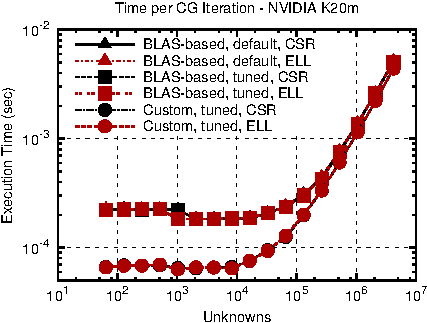
\includegraphics[width=0.85\textwidth]{figures/cg-k20m-3}
 \end{center}

 \begin{itemize}
  \item   \vspace*{-0.3cm} {\small (2D Finite Difference Discretization)}
 \end{itemize}
 \end{block}   
\end{frame}

\begin{frame}[fragile]{Conjugate Gradients}
 \begin{block}{}
 \begin{center}
  \vspace*{-0.5cm}
  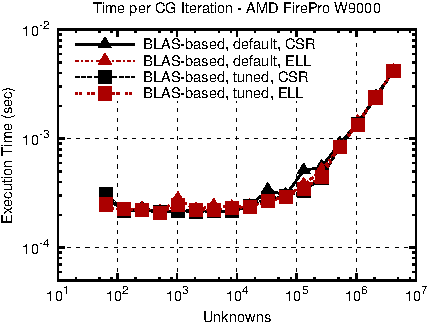
\includegraphics[width=0.85\textwidth]{figures/cg-firepro-w9000-2}
 \end{center}

 \begin{itemize}
  \item   \vspace*{-0.3cm} {\small (2D Finite Difference Discretization)}
 \end{itemize}
 \end{block}   
\end{frame}

\begin{frame}[fragile]{Conjugate Gradients}
 \begin{block}{}
 \begin{center}
  \vspace*{-0.5cm}
  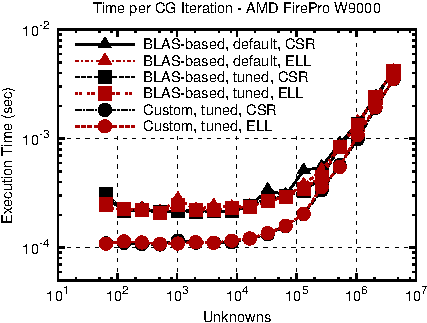
\includegraphics[width=0.85\textwidth]{figures/cg-firepro-w9000-3}
 \end{center}

 \begin{itemize}
  \item   \vspace*{-0.3cm} {\small (2D Finite Difference Discretization)}
 \end{itemize}
 \end{block}   
\end{frame}



%%% BiCGStab and GMRES optimization:


\begin{frame}{Outline}
 \begin{center}
  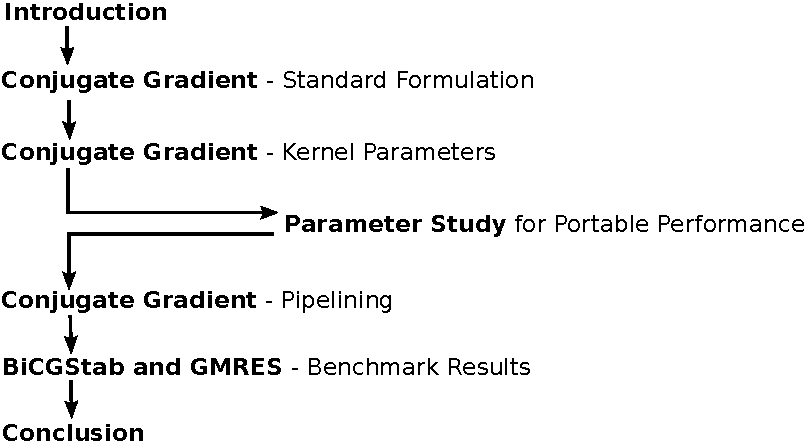
\includegraphics[width=0.9\textwidth]{figures/outline-crop}
 \end{center}
\end{frame}


\begin{frame}[fragile]{BiCGStab and GMRES}
 \begin{block}{BiCGStab}
 \begin{itemize}
  \item Similar to CG
  \item Two SpMV per iteration
  \item Pipelining: 4 kernel launches instead of 12
 \end{itemize}
 \end{block}   
 
 \begin{block}{GMRES}
 \begin{itemize}
  \item Store Krylov basis
  \item Orthonormalization in each step
  \item Pipelining: 3 kernel launches
 \end{itemize}
 \end{block}   

 \begin{block}{Benchmark Setup}
 \begin{itemize}
  \item Poisson equation in 2D
  \item GPUs from NVIDIA and AMD
 \end{itemize}
 \end{block}   

\end{frame}



\begin{frame}[fragile]{BiCGStab Benchmarks}
 \begin{block}{}
 \begin{center}
  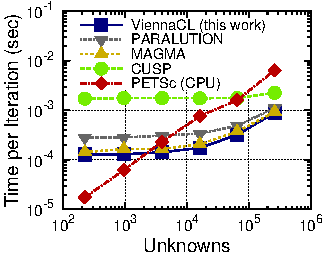
\includegraphics[width=0.7\textwidth]{figures/time-laplace2d-K20m-bicgstab}
 \end{center}
 \end{block}   
\end{frame}

\begin{frame}[fragile]{BiCGStab Benchmarks}
 \begin{block}{}
 \begin{center}
  \vspace*{-1cm}
  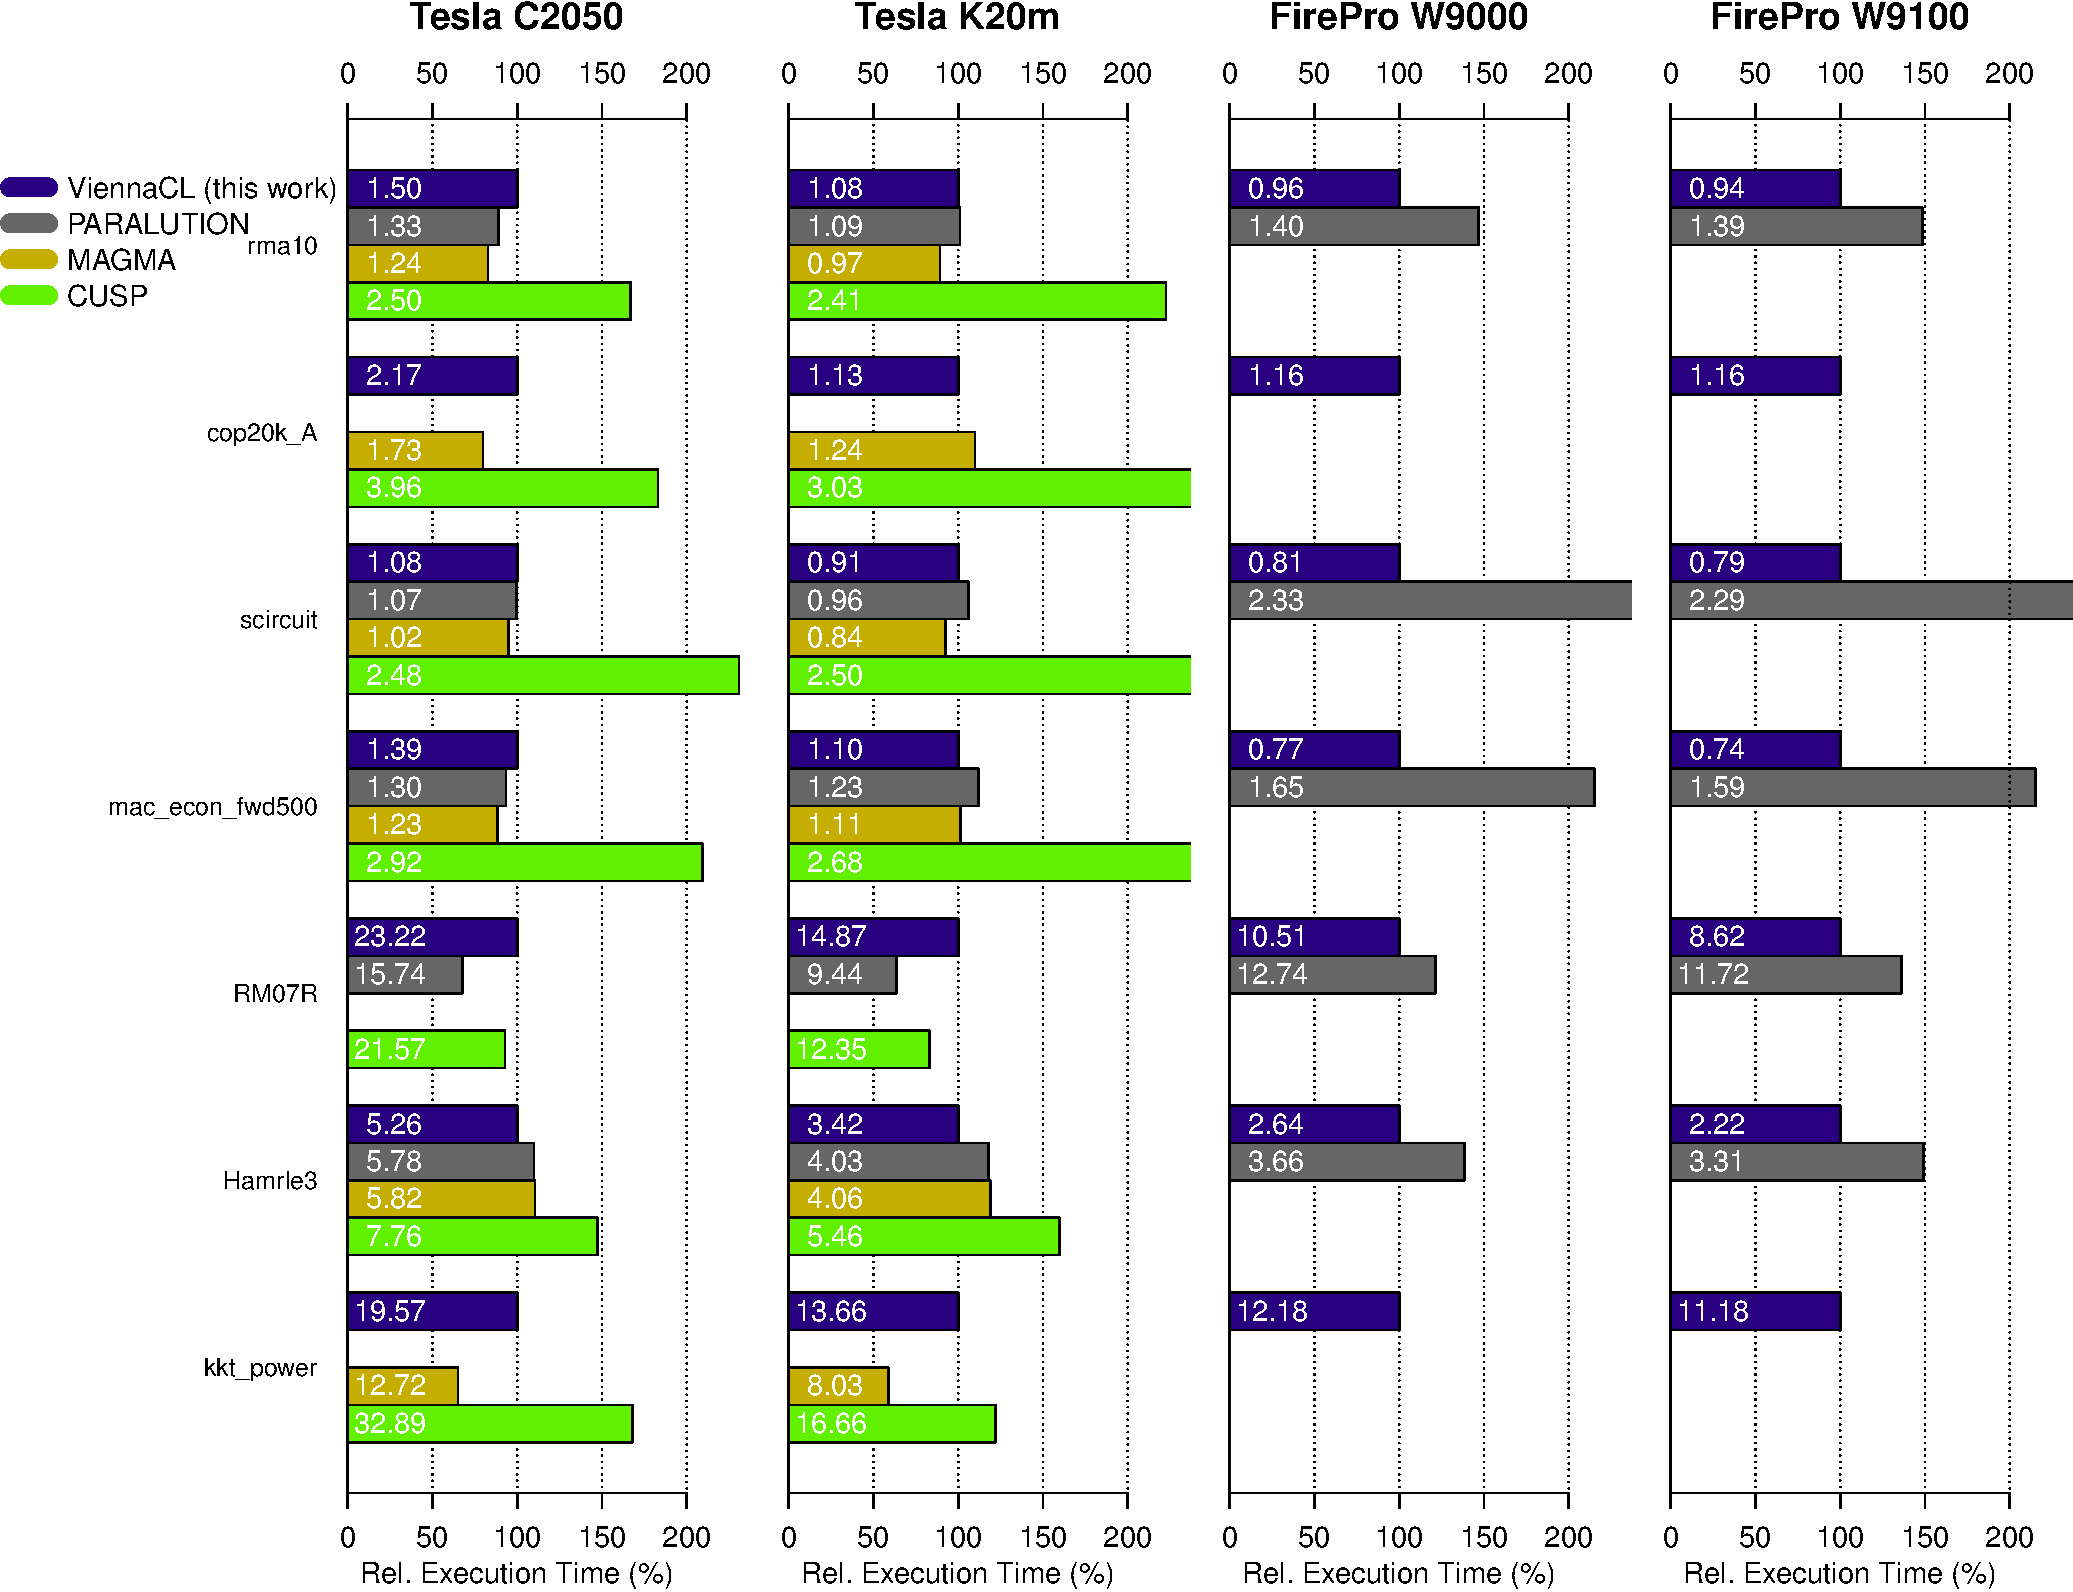
\includegraphics[width=0.9\textwidth]{figures/bicgstab}
 \end{center}
 \end{block}   
\end{frame}

\begin{frame}[fragile]{GMRES Benchmarks}
 \begin{block}{}
 \begin{center}
  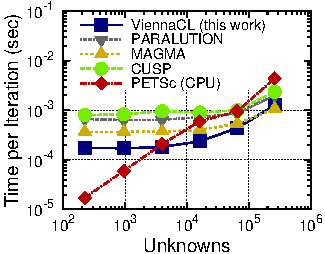
\includegraphics[width=0.7\textwidth]{figures/time-laplace2d-K20m-gmres}
 \end{center}
 \end{block}   
\end{frame}

\begin{frame}[fragile]{GMRES Benchmarks}
 \begin{block}{}
 \begin{center}
  \vspace*{-1cm}
  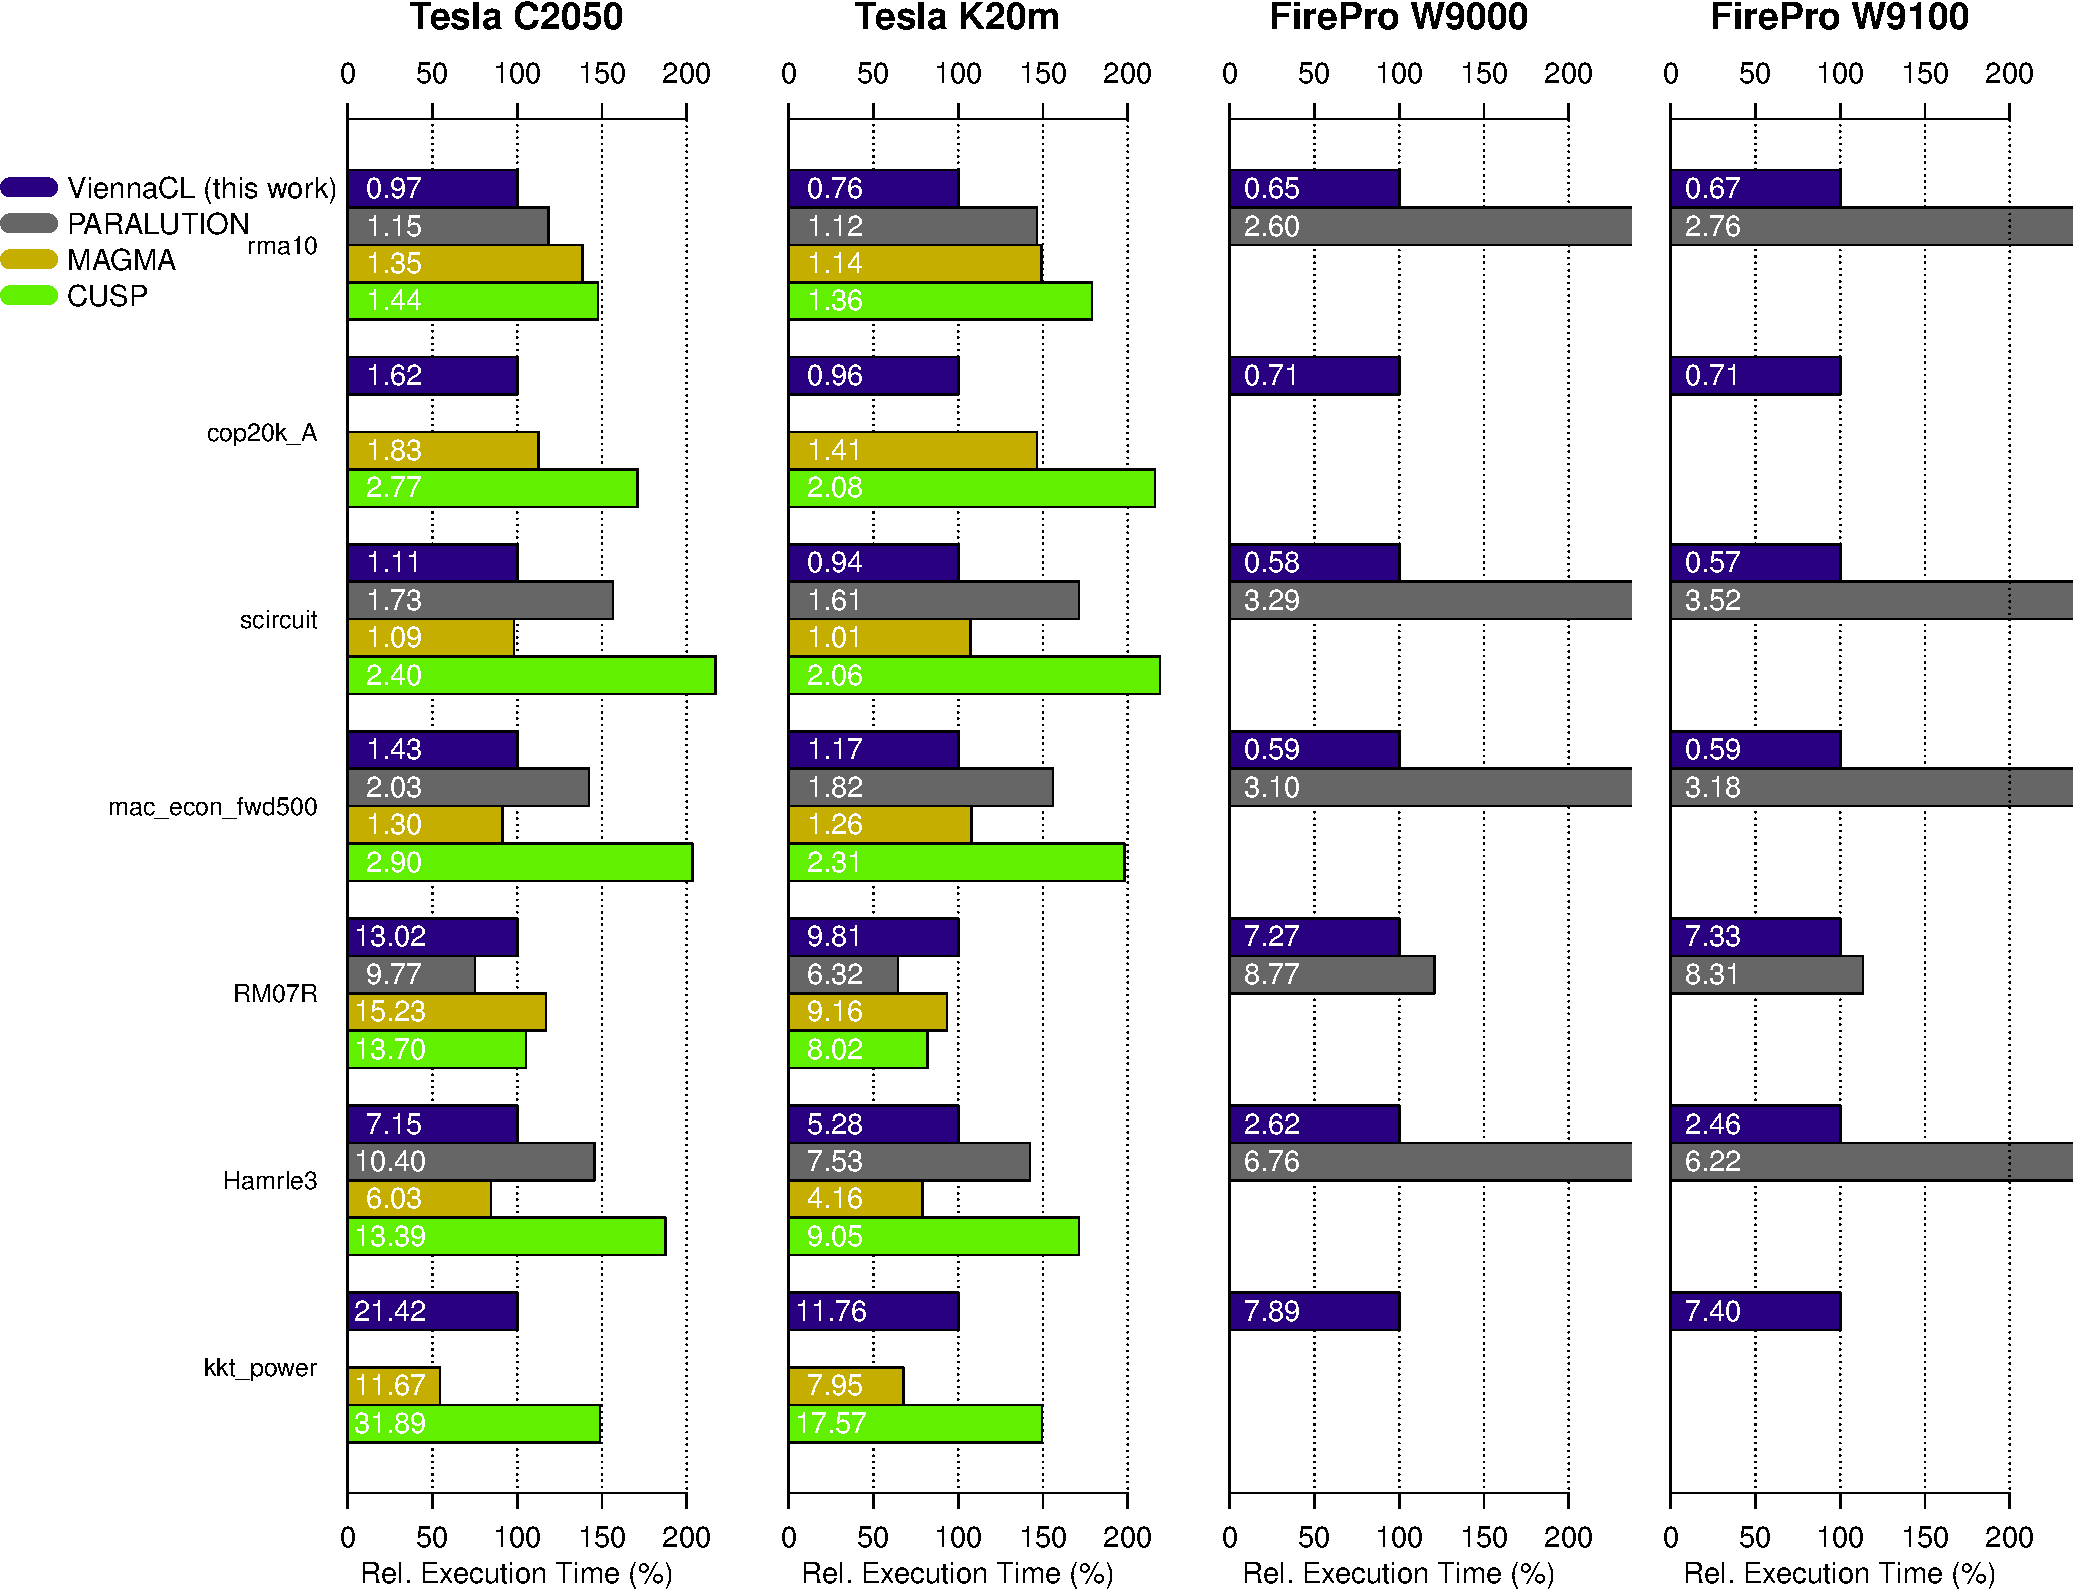
\includegraphics[width=0.9\textwidth]{figures/gmres}
 \end{center}
 \end{block}   
\end{frame}




%
% Discuss BiCGStab and GMRES performance results:
%

%%% GMRES optimization:
% mdot


\begin{frame}[fragile]{GMRES Optimization}

 \begin{block}{Generalized Minimum Residual (GMRES) Method}
   \begin{itemize}
    \item Krylov space  $\mathrm{span}\{r, Ar, A^2r, \ldots, A^{N-1}r\}$
    \item Orthogonal basis $\{v_1, v_2, \ldots, v_N\}$
   \end{itemize}
 \end{block}

 %\pause
 \begin{block}{Gram-Schmidt Method revisited}
   \begin{itemize}
    \item Given: orthonormal basis $\{v_1, v_2, \ldots, v_N\}$, augment by $w$
    \item $w \leftarrow w - \sum_{i=1}^N \langle w, v_i \rangle v_i$
    \item $w \leftarrow w / \Vert w \Vert$
    \item Add $w$ to basis
   \end{itemize}
 \end{block}

 %\pause
 \begin{block}{Multiple inner products $\langle w, v_i \rangle$}
   \begin{itemize}
    \item Performance critical (global reductions)
    \item Reuse of $w$ desirable
   \end{itemize}
 \end{block}
\end{frame}


% - mdot
\begin{frame}[fragile]{GMRES Optimization}

 \begin{block}{Custom routine \textit{mdot}}
   \begin{itemize}
    \item Process $\alpha_i = \langle w, v_i \rangle$ in batches
    \item Batch sizes 1, 2, 3, 4, 8
    \item Batch size 8: Only $12.5 \%$ overhead vs.~arbitrary batch sizes
   \end{itemize}
 \end{block}

 \begin{block}{Code sketch (Batch size 4)}
 \begin{lstlisting}
 for (size_t i=thread_id; i<M; i += threads_per_group)
 {
   double val_w = w[i];
   alpha_1 += val_w * v1[i];
   alpha_2 += val_w * v2[i];
   alpha_3 += val_w * v3[i];
   alpha_4 += val_w * v4[i];
 }
   \end{lstlisting}
 \end{block}
    

\end{frame}

\begin{frame}{Benchmarks}
 \begin{center}
   \centering 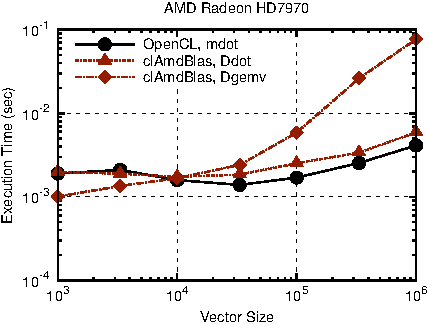
\includegraphics[width=0.8\textwidth]{figures/time-size-amd-3} \\[1em]
   \hspace*{1cm} Fixed number of $50$ vectors
 \end{center}
\end{frame}

\begin{frame}{Benchmarks}
 \begin{center}
   \centering 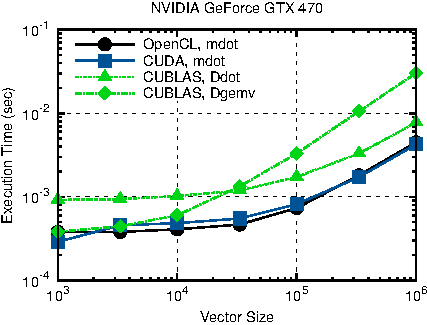
\includegraphics[width=0.8\textwidth]{figures/time-size-nvidia-4} \\[1em]
   \hspace*{1cm} Fixed number of $50$ vectors
 \end{center}
\end{frame}





%
% Conclusion:
%

\begin{frame}{Conclusion}

  \begin{block}{Performance-Portable Code for GPUs}
    \begin{itemize}
     \item Start with 128 work items
     \item Refrain from using vector datatypes
     \item Let each workgroup work on a contiguous piece of memory
    \end{itemize}
  \end{block}

  \begin{block}{Pipelined Iterative Solvers}
    \begin{itemize}
     \item Reduced number of kernel launches
     \item On-chip data reuse
     \item Faster than BLAS-based implementations
    \end{itemize}
  \end{block}

  \begin{block}{Best Practices for GPU Computing}
    \begin{itemize}
      \item FLOPs are (almost always) for free
      \item Work on large enough data
      \item Avoid unnecessary PCI-Express communication
    \end{itemize}
  \end{block}

\end{frame}


